% Question Objectives
% - Functions that are rebound to a different variable still have the same
%   intrinsic name.

\begin{blocksection}
\question Draw the environment diagram that results from executing the
code below. What will be displayed when running the code (note this separately 
from the diagram)?

\begin{lstlisting}
from operator import add
def sub(a, b):
    sub = add
    return a - b
add = sub
sub = min
print(add(2, sub(2, 3)))
\end{lstlisting}

\begin{solution}[2.5in]
\begin{center}
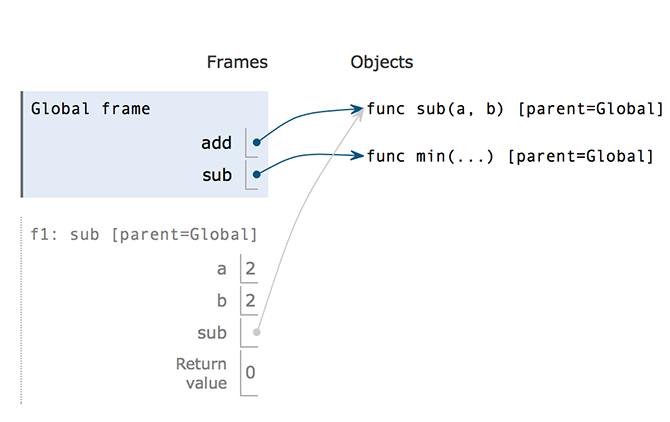
\includegraphics{add-sub.png}
\begin{lstlisting}
Print output:
0
\end{lstlisting}
\end{center}
\href{https://www.youtube.com/watch?v=Fiw0f5yuQgo&vq=hd1080&t=59m22s}{Video walkthrough}
\end{solution}
\end{blocksection}
